\chapter{Linear Regression}   
\label{chap:linreg}

In many senses, this chapter and several of the following ones form the
real core of statistics, especially from a computer science point of
view.

In this chapter and the next, we are interested in relations between
variables, in two main senses:

\begin{itemize}

\item In {\bf regression analysis}, we are interested in the relation of
one variable with one or more others.

\item In other kinds of analyses, such as {\bf principal components
analysis}, we are interested in relations among several variables,
symmetrically, i.e. not having one variable play a special role.

\end{itemize}

Note carefully that {\it many types of methods that go by another name
are actually regression methods}.  Examples are the {\bf classification
problem}, {\bf discriminant analysis}, {\bf pattern recognition}, {\bf
machine learning} and so on.  We'll return to this point in Chapter
\ref{chap:class}.

\section{The Goals:  Prediction and Description}
\label{goals}

{\it Prediction is difficult, especially when it's about the
future.}---Yogi Berra\footnote{Yogi Berra (1925-2015) is a former baseball
player and manager, famous for his malapropisms, such as ``When you
reach a fork in the road, take it''; ``That restaurant is so crowded
that no one goes there anymore''; and ``I never said half the things I
really said.''} 

\bigskip

Before beginning, it is important to understand the typical goals in
regression analysis.

\begin{itemize}

\item {\bf Prediction:}  Here we are trying to predict one variable from
one or more others.

\item {\bf Description:}  Here we wish to determine which of several
variables have a greater effect on (or relation to) a given variable.
An important special case is that in which we are interested in
determining the effect of one predictor variable, {\bf after the effects
of the other predictors are removed.}

\end{itemize}

Denote the {\bf predictor variables} by, $X^{(1)},...,X^{(r)}$, alluding
to the Prediction goal.  They are also called {\bf independent
variables} or {\bf explanatory variables} (the latter term highlighting
the Description goal) The variable to be predicted, Y, is often called
the {\bf response variable}, or the {\bf dependent variable}.  Note that
one or more of the variables---whether the predictors or the response
variable---may be indicator variables (Section \ref{indicator}).
Another name for response variables of that type is {\bf dummy
variables}.  

Methodology for this kind of setting is called {\bf regression
analysis}.  If the response variable Y is an indicator variable, the
values 1 and 0 to indicate class membership, we call this the {\bf
classification problem}.  (If we have more than two classes, we need
several Ys.)

In the above context, we are interested in the relation of a single
variable Y with other variables $X^{(i)}$.  But in some applications, we
are interested in the more symmetric problem of relations {\it among}
variables $X^{(i)}$ (with there being no Y).  A typical tool for the
case of continuous random variables is {\bf principal components
analysis}, and a popular one for the discrete case is {\bf log-linear
model}; both will be discussed later in this chapter.

\section{Example Applications:  Software Engineering, Networks, Text
Mining}
\label{examples}

{\bf Example:}  As an aid in deciding which applicants to admit to a
graduate program in computer science, we might try to predict Y, a
faculty rating of a student after completion of his/her first year in
the program, from $X^{(1)}$ = the student's CS GRE score, $X^{(2)}$ = the
student's undergraduate GPA and various other variables.  Here our goal
would be Prediction, but educational researchers might do the same thing
with the goal of Description.  For an example of the latter, see
Predicting Academic Performance in the School of Computing \& Information
Technology (SCIT), {\it 35th ASEE/IEEE Frontiers in Education
Conference}, by Paul Golding and Sophia McNamarah, 2005.

{\bf Example:}  In a paper, Estimation of Network Distances Using
Off-line Measurements, {\it Computer Communications}, by Prasun Sinha,
Danny Raz and Nidhan Choudhuri, 2006, the authors wanted to predict Y,
the round-trip time (RTT) for packets in a network, using the predictor
variables $X^{(1)}$ = geographical distance between the two nodes,
$X^{(2)}$ = number of router-to-router hops, and other offline
variables.  The goal here was primarily Prediction.

{\bf Example:}  In a paper, Productivity Analysis of Object-Oriented
Software Developed in a Commercial Environment, {\it Software---Practice
and Experience}, by Thomas E. Potok, Mladen Vouk and Andy Rindos, 1999,
the authors mainly had an Description goal:  What impact, positive or
negative, does the use of object-oriented programming have on programmer
productivity?  Here they predicted Y = number of person-months needed to
complete the project, from  $X^{(1)}$ = size of the project as measured
in lines of code,  $X^{(2)}$ = 1 or 0 depending on whether an
object-oriented or procedural approach was used, and other variables.

{\bf Example:}  Most {\bf text mining} applications are classification
problems.  For example, the paper Untangling Text Data Mining, {\it
Proceedings of ACL'99}, by Marti Hearst, 1999 cites, {\it inter alia},
an application in which the analysts wished to know what proportion of
patents come from publicly funded research.  They were using a patent
database, which of course is far too huge to feasibly search by hand.
That meant that they needed to be able to (reasonably reliably) predict
Y = 1 or 0, according to whether the patent was publicly funded from a
number of $X^{(i)}$, each of which was an indicator variable for a given
key word, such as ``NSF.''  They would then treat the predicted Y values
as the real ones, and estimate their proportion from them.

{\bf Example:} A major health insurance company wanted to have a tool to
predict which of its members would be likely to need hospitalization in
the next year.  Here Y = 1 or 0, according to whether the patient turns
out to be hospitalized, and the predictor variables were the members'
demographics, previous medical history and so on.  (Interestingly,
rather hiring its own data scientist to do the analysis, the company put
the problem on Kaggle, a site that holds predictive analytics
competitions, \url{www.kaggle.com}.)

\section{Adjusting for Covariates}

The first statistical consulting engagement I ever worked involved
something called {\it adjusting for covariates}.  I was retained by the
Kaiser hospital chain to investigate how heart attack patients fared at
the various hospitals---did patients have a better chance to survive in
some hospitals than in others?  There were four hospitals of particular
interest.

I could have simply computed raw survival rates, say the proportion of
patients who survive for a month following a heart attack, and then used
the methods of Section \ref{propcis}, for instance.  This could have
been misleading, though, because one of the four hospitals served a
largely elderly population.  A straight comparison of survival rates
might then unfairly paint that particular hospital as giving lower
quality of care than the others.

So, we want to somehow adjust for the effects of age.  I did this by
setting Y to 1 or 0, for survival, $X^{(1)}$ to age, and $X^{(2+i)}$ to be
an indicator random variable for whether the patient was at hospital i,
i = 1,2,3.\footnote{Note that there is no i = 4 case, since if the first
three hospital variables are all 0, that already tells us that this
patient was at the fourth hospital.}

\section{What Does ``Relationship'' Really Mean?}
\label{regintro}

Consider the Davis city population example again.  In addition to the
random variable $W$ for weight, let $H$ denote the person's height.
Suppose we are interested in exploring the relationship between height
and weight.

As usual, we must first ask, {\bf what does that really mean}?  What do
we mean by ``relationship''?  Clearly, there is no exact relationship;
for instance, a person's weight is not an exact function of his/her
height.

Effective use of the methods to be presented here requires an
understanding of what exactly is meant by the term {\it relationship} in
this context.

\subsection{Precise Definition}

Intuitively, we would guess that mean weight increases with
height.  To state this precisely, the key word in the previous sentence
is {\it mean}.

Take Y to be the weight W and $X^{(1)}$ to be the height H, and define

\begin{equation}
\label{firstreg}
m_{W;H}(t) = E(W|H = t)
\end{equation}

This looks abstract, but it is just common-sense stuff.  For example,
$m_{W;H}(68)$ would be the mean weight of all people in the population
of height 68 inches.  The value of $m_{W;H}(t)$ varies with t, and we
would expect that a graph of it would show an increasing trend with t,
reflecting that taller people tend to be heavier.  

We call $m_{W;H}$ the {\bf regression function of W on H}.  In general,
$m_{Y;X}(t)$ means the mean of $Y$ among all units in the population for
which $X = t$.\footnote{The word ``regression'' is an allusion to the
famous comment of Sir Francis Galton in the late 1800s regarding
``regression toward the mean.''  This referred to the fact that tall
parents tend to have children who are less tall---closer to the
mean---with a similar statement for short parents.  The predictor
variable here might be, say, the father's height F, with the response
variable being, say, the son's height S.  Galton was saying that 
E(S $|$ F) $<$ F.}

Note the word {\it population} in that last sentence.  The function m()
is a \underline{population} function.

So we have:

\begin{quote}
{\bf Major Point 1:} When we talk about the {\it relationship} of one
variable to one or more others, we are referring to the regression function,
which expresses the mean of the first variable as a function of the
others.  The key word here is {\it mean}!
\end{quote}

\subsection{(Rather Artificial) Example:  Marble Problem}

Recall the marble selection example in Section \ref{marblepmf}:  Suppose
we have a bag containing two yellow marbles, three blue ones and four
green ones.  We choose four marbles from the bag at random, without
replacement.  Let Y and B denote the number of yellow and blue marbles
that we get.  Let's find  $m_{Y;B}(2)$.

For convenience, Table \ref{marblepmf1} shows what we found before for P(Y = i and B = j).

\begin{table}
\vskip 0.5in
\vskip 0.5in
\begin{center}
\begin{tabular}{|r|r|r|r|r|r|}
\hline
i $\downarrow$, j $\rightarrow$ & 0 & 1 & 2 & 3 \\ \hline
0 & 0.0079 & 0.0952 & 0.1429 & 0.0317 \\ \hline
1 & 0.0635 & 0.2857 & 0.1905 & 0.1587 \\ \hline
2 & 0.0476 & 0.0952 & 0.0238 & 0.000 \\ \hline
\end{tabular}
\end{center}
\caption{Bivariate pmf for the Marble Problem}
\label{marblepmf1}
\end{table}


Now keep in mind that since $m_{Y;B}(t)$ is the conditional mean of Y
given B, we need to use conditional probabilities to compute it.  For
our example here of $m_{Y;B}(2)$, we need the probabilities $P(Y = k | B
= 2)$.  For instance,

\begin{eqnarray}
P( Y = 1 | B = 2) &=& \frac{p_{Y,B}(1,2)}{p_B(2)} \\ 
&=& \frac{0.1905}{0.1492 + 0.1905 + 0.0238} \\
&=& 0.5333
\end{eqnarray}

The other conditional $P(Y = k | B = 2)$ are then found to be 
0.1429/0.3572 = 0.4001 for k = 0 and
0.0238/0.3572 = 0.0667 for k = 2. 

\begin{equation}
m_{Y;B}(2) = 0.4001 \cdot 0 + 0.5333 \cdot 1 + 0.0667 \cdot 2 = 0.667
\end{equation}

\section{Estimating That Relationship from Sample Data}
\label{estfromsample}

The marble example in the last section was rather artificial, in that
the exact distribution of the variables was known (Table
\ref{marblepmf1}).  In real applications, we don't know this
distribution, and must estimate it from sample data.

As noted, $m_{W;H}(t)$ is a \underline{population} function,
dependent on \underline{population} distributions.  How can we estimate
this function from sample data?

Toward that end, let's again suppose we have a random sample of 1000
people from Davis, with 

\begin{equation}
(H_1,W_1),...,(H_{1000},W_{1000})
\end{equation}

being their heights and weights.  We again wish to use this data to
estimate population values, meaning the population regression function
of W on H, $m_{W;H}(t)$.  But the difference here is that we are
estimating a whole function now, the whole curve $m_{W;H}(t)$.  That
means we are estimating infinitely many values, with one $m_{W;H}(t)$
value for each t.\footnote{Of course, the population of Davis is finite,
but there is the conceptual population of all people who {\it could}
live in Davis.} How do we do this?

One approach would be as follows.  Say we wish to find
$\widehat{m}_{W;H}(t)$ (note the hat, for ``estimate of''!) at t = 70.2.
In other words, we wish to estimate the mean weight---in the
population---among all people of height 70.2.  What we could do is look
at all the people in our sample who are within, say, 1.0 inch of 70.2,
and calculate the average of all their weights.  This would then be our
$\widehat{m}_{W;H}(t)$. 

\subsection{Parametric Models for the Regression Function m()}

There are many methods like the above (Chapter \ref{chap:nonparregclass}),
but the traditional method is to choose a parametric model for the
regression function.  That way we estimate only a finite number of
quantities instead of an infinite number.  This would be good in light
of Section \ref{dfd}.

Typically the parametric model chosen is linear, i.e.  we assume that
$m_{W;H}(t)$ is a linear function of t:

\begin{equation}
\label{par}
m_{W;H}(t) = ct+d
\end{equation}

for some constants c and d.  If this assumption is reasonable---meaning
that though it may not be exactly true it is reasonably close---then it
is a huge gain for us over a nonparametric model.  Do you see why?
Again, the answer is that instead of having to estimate an infinite
number of quantities, we now must estimate only two quantities---the
parameters c and d.

Equation (\ref{par}) is thus called a {\bf parametric} model of
$m_{W;H}()$.  The set of straight lines indexed by c and d is a
two-parameter family, analogous to parametric families of distributions,
such as the two-parametric gamma family; the difference, of course, is
that in the gamma case we were modeling a density function, and here we
are modeling a regression function.

Note that c and d are indeed population parameters in the same sense
that, for instance, r and $\lambda$ are parameters in the gamma
distribution family.  We must estimate c and d from our sample data.

So we have:

\begin{quote}
{\bf Major Point 2:}  The function $m_{W;H}(t)$ is a population entity,
so we must estimate it from our sample data.  To do this, we have a 
choice of either assuming that $m_{W;H}(t)$ takes on some parametric 
form, or making no such assumption.

If we opt for a parametric approach, the most common model is linear,
i.e. (\ref{par}).  Again, the quantities c and d in (\ref{par}) are
population values, and as such, we must estimate them from the data.

\end{quote}

\subsection{Estimation in Parametric Regression Models}

So, how can we estimate these population values c and d?  We'll go into
details in Section \ref{parest}, but here is a preview:

\label{optimpred}
Using the result on page \pageref{mingcpage}, together with the
principle of iterated expectation, (\ref{adamsdiscrete}) and
(\ref{adamscontin}), we can show that the minimum value of the quantity

\begin{equation}
E \left [ \left ( W - g(H) \right )^2 \right ]
\end{equation}

overall all possible functions $g(H)$, is attained by setting

\begin{equation}
g(H) = m_{W;H}(H)
\end{equation}

In other words, $m_{W;H}(H)$ is the optimal predictor of W among all
possible functions of H, in the sense of minimizing mean squared
prediction error.\footnote{But if we wish to minimize the mean absolute
prediction error, $E \left ( | W - g(H) | \right )$, the best function
turns out to be is $g(H) = \textrm{median}(W|H)$.}  

Since we are assuming the model (\ref{par}), this in turn means that:

\begin{quote}

The quantity 

\begin{equation}
\label{rspe}
E \left [ \left ( W - (uH+v) \right )^2 \right ]
\end{equation}

is minimized by setting u = c and v = d.  

\end{quote}

This then gives us a clue as to how to estimate c and d from our data,
as follows.

If you recall, in earlier chapters we've often chosen estimators by
using sample analogs, e.g.  $s^2$ as an estimator of $\sigma^2$.  Well,
the sample analog of (\ref{rspe}) is

\begin{equation}
\label{srspe}
\frac{1}{n} \sum_{i=1}^n \left [ W_i - (uH_i + v) \right ]^2
\end{equation}

Here (\ref{rspe}) is the mean squared prediction error using u and v in
the population, and (\ref{srspe}) is the mean squared prediction error
using u and v in our sample.  Since u = c and v = d minimize
(\ref{rspe}), it is natural to estimate c and d by the u and v that
minimize (\ref{srspe}).  

Using the ``hat'' notation common for estimators, we'll denote the u and
v that minimize (\ref{srspe}) by $\hat{c}$ and $\hat{d}$, respectively.
These numbers are then the classical {\bf least-squares
estimators} of the population values c and d.

\begin{quote}
{\bf Major Point 3:}  In statistical regression analysis, one uses a
linear model as in (\ref{par}), estimating the coefficients by
minimizing (\ref{srspe}).
\end{quote}

We will elaborate on this in Section \ref{parest}.

\subsection{More on Parametric vs. Nonparametric Models}

Suppose we're interested in the distribution of battery lifetimes, and
we have a sample of them, say $B_1,...,B_{100}$.  We wish to estimate
the density of lifetimes in the population of all batteries of this
kind, $f_B(t)$.

We have two choices:

\begin{itemize}

\item [(a)] We can simply plot a histogram of our data, which we found
in Chapter \ref{chap:nonpardens} is actually a density estimator.  We
are estimating infinitely many population quantities, namely the heights
of the curve $f_B(t)$ at infinitely many values of t.

\item [(b)] We could postulate a model for the distribution of battery
lifetime, say using the gamma family (Section \ref{gammafam}).  Then we
would estimate just two parameters, $\lambda$ and $r$.

\end{itemize}

What are the pros and cons of (a) versus (b)?  The approach (a) is nice,
because we don't have to make any assumptions about the form of the
curve $f_B(t)$; we just estimate it directly, with the histogram or
other method from Chapter \ref{chap:nonpardens}.  But we are, in
essence, using a finite amount of data to estimate an infinite values.

As to (b), it requires us to estimate only two parameters, which is
nice.  Also, having a nice, compact parametric form for our estimate is
appealing.  But we have the problem of having to make an assumption
about the form of the model.  We then have to see how well the model
fits the data, say using the methods in Chapter \ref{chap:mod}.  If it
turns out not to fit well, we may try other models (e.g. from the
Weibull family, not presented in this book).

The above situation is exactly parallel to what we are studying in the
present chapter.  The analogy here of estimating a density function is
estimating a regression function.  The analog of the histogram in (a) is
the ``average the people near a given height'' method.  The analog here
of using a parametric family of densities, such as the gamma, is using a
parametric family of straight lines.  And the analog of comparing
several candidate parametric density models is to compare several
regression models, e.g. adding quadratic or cubic terms ($t^2$, $t^3$)
for height in (\ref{par}).  (See Section \ref{diags} for reading on
model assessment methods.)

Most statistical analysts prefer parameteric models, but nonparametric
approaches are becoming increasingly popular.

\section{Example:  Baseball Data}
\label{baseball1}

Let's do a regression analysis of weight against height in the baseball
player data introduced in Section \ref{baseball0}.

\subsection{R Code}

I ran R's {\bf lm()} (``linear model'') function to perform the
regression analysis:

\begin{verbatim}
> summary(lm(players$Weight ~ players$Height))

Call:
lm(formula = players$Weight ~ players$Height)

Residuals:
    Min      1Q  Median      3Q     Max 
-51.988 -13.147   1.218  11.694  70.012 

Coefficients:
               Estimate Std. Error t value Pr(>|t|)    
(Intercept)    -155.092     17.699  -8.763   <2e-16 ***
players$Height    4.841      0.240  20.168   <2e-16 ***
---
Signif. codes:  0 ‘***’ 0.001 ‘**’ 0.01 ‘*’ 0.05 ‘.’ 0.1 ‘ ’ 1 

Residual standard error: 17.78 on 1031 degrees of freedom
  (1 observation deleted due to missingness)
Multiple R-squared: 0.2829,	Adjusted R-squared: 0.2822 
F-statistic: 406.7 on 1 and 1031 DF,  p-value: < 2.2e-16 
\end{verbatim}

\label{asterisksexample}

This illustrates the {\bf polymorphic} nature of R:  The same
function can be applied to different classes of objects.  Here {\bf
summary()} is such a function; another common one is {\bf plot()}.  So,
we can call {\bf summary()} on an object of any class, at least, any one
for which a {\bf summary()} function has been written.  In the above R
output, we called {\bf summary()} on an object of type {\bf "lm"}; the R
interpreter checked the class of our object, and then accordingly called
{\bf summary.lm()}.  But it's convenient for us, since we ignore all
that and simply call {\bf summary()} no matter what our object is.

The call \lstinline{lm(players$Weight ~ players$Height)} specified that
my response and predictor variables were the Weight and Height columns
in the {\bf players} data frame.  

{\bf Note:}  The variables here are specified in an R data frame.  One
can also specify via a matrix, which gives more flexibility.  For
example, 

\begin{lstlisting}
lm(y ~ x[,c(2,3,7)])
\end{lstlisting}

to predict {\bf y} from columns 2, 3 and 7 of {\bf x}.

\subsection{A Look through the Output}

Next, note that {\bf lm()} returns a lot of information (even more than
shown above), all packed into an object of type {\bf "lm"}.\footnote{R
class names are quoted.}  By calling {\bf summary()} on that object, I
got some of the information.  It gave me more than we'll cover for
now, but the key is that it told me that the sample estimates of c and d
are 

\begin{equation}
\hat{d} = -155.092
\end{equation}

\begin{equation}
\hat{c} = 4.841
\end{equation}

In other words, our estimate for the function giving mean weight in
terms of height is

\begin{lstlisting}
mean weight = -155.092 + 4.841 height
\end{lstlisting} 

Do keep in mind that this is just an estimate, based on the sample data;
it is not the population mean-weight-versus-height function.  So for
example, our {\it sample estimate} is that an extra inch in height
corresponds on average to about 4.8 more pounds in weight.  

We can form a confidence interval to make that point clear, and get an
idea of how accurate our estimate is.  The R output tells us that the
standard error of $\hat{d}$ is 0.240.  Making use of Section \ref{stderrest},
we add and subtract 1.96 times this number to $\hat{d}$ to get our interval:
(4.351,5.331).  So, we are about 95\% confident that the true slope, c,
is in that interval.

Note the column of output labled ``t value.''  This is again a Student-t
test, with the p-value given in the last column, labeled ``$Pr( >
|t|)$.''  Let's discuss this.  In the row of the summary above regarding
the Height variable, for example, we are testing

\begin{equation}
\label{h0c}
H_0:  c = 0
\end{equation}

R is using a Student-t distribution for this, while we have been using the
the N(0,1) distribution, based on the Central Limit Theorem
approximation.  For all but the smallest samples, the difference is
negligible.  Consider:

Using (\ref{genz}), we would test (\ref{h0c}) by forming the quotient

\begin{equation}
\frac{4.841 - 0}{0.240} = 20.17
\end{equation}

This is essentially the same as the 20.168 we see in the above summary.
In other words, don't worry that R uses the Student-t distribution while
we use (\ref{genz}).

At any rate, 20.17 is way larger than 1.96, thus resulting in rejection
of $H_0$.  The p-value is then the area to the left of -20.17 and to the
right of 20.17, which we could compute using {\bf pnorm()}.  But R has
already done this for us, reporting that the p-value is $2 \times
10^{-16}$.

What about the {\bf residuals}?  Here we go back to the original
$(H_i,W_i)$ data with our slope and intercept estimates, and ``predict''
each $W_i$ from the corresponding $H_i$.  The residuals are the
resulting prediction errors.  In other words, the i$^{th}$ residual is

\begin{equation}
W_i - (\hat{d} + \hat{c} H_i)
\end{equation}

You might wonder why we would try to predict the data that we already
know!  But the reason for doing this is to try to assess how well we can
predict future cases, in which we know height but not weight.  If we can
``predict'' well in our known data, maybe we'll do well later with
unknown data.  This will turn out to be somewhat overoptimistic, we'll
see, but again, the residuals should be of at least {\it some} value in
assessing the predictive ability of our model.  So, the R output reports
to us what the smallest and largest residual values were.

The $R^2$ values will be explained in Section \ref{varsel}.

Finally, the F-test is a significance test that c = d = 0.  Since this
book does not regard testing as very useful, this aspect will not be
pursued here.

% \checkpoint

\section{Multiple Regression:  More Than One Predictor Variable}

Note that $X$ and t could be vector-valued.  For instance, we could have
$Y$ be weight and have $X$ be the pair 

\begin{equation}
X = \left ( X^{(1)},X^{(2)} \right ) = (H,A) = \textrm{(height, age)} 
\end{equation}

so as to study the relationship of weight with height and age.  If we
used a linear model, we would write for $t = (t_1,t_2)$,

\begin{equation}
\label{heightage}
m_{W;H,A}(t) = \beta_0 + \beta_1 t_1 + \beta_2 t_2
\end{equation}

In other words

\begin{equation}
\label{wthtage}
\textrm{mean weight} = \beta_0 + \beta_1 \textrm{ height} + 
\beta_2 \textrm{ age}
\end{equation}

Once again, keep in mind that (\ref{heightage}) and (\ref{wthtage}) are
models for the \underline{population}.  We assume that
(\ref{heightage}), (\ref{wthtage}) or whichever model we use is an exact
representation of the relation in the population.  And of course, our
derivations below assume our model is correct.

(It is traditional to use the Greek letter $\beta$ to name the
coefficients in a linear regression model.)

So for instance $m_{W;H,A}(68,37.2)$ would be the mean weight in the
population of all people having height 68 and age 37.2.

In analogy with (\ref{srspe}), we would estimate the $\beta_i$ by
minimizing

\begin{equation}
\label{srspe2}
\frac{1}{n} \sum_{i=1}^n \left [ W_i - (u+vH_i+wA_i) \right ]^2
\end{equation}

with respect to u, v and w.  The minimizing values would be denoted
$\widehat{\beta}_0$, $\widehat{\beta}_1$ and $\widehat{\beta}_2$.

We might consider adding a third predictor, gender:

\begin{equation}
\label{wthtagegender}
\textrm{mean weight} = \beta_0 + \beta_1 \textrm{ height} + 
\beta_2 \textrm{ age} + \beta_3 \textrm{ gender}
\end{equation}

where {\bf gender} is an indicator variable, 1 for male, 0 for female.
Note that we would not have two gender variables, since knowledge of the
value of one such variable would tell us for sure what the other one is.
(It would also make a certain matrix noninvertible, as we'll discuss
later.)

\section{Example:  Baseball Data (cont'd.)}
\label{baseball2}

So, let's regress weight against height and age:

\begin{verbatim}
> summary(lm(players$Weight ~ players$Height + players$Age))

Call:
lm(formula = players$Weight ~ players$Height + players$Age)

Residuals:
    Min      1Q  Median      3Q     Max 
-50.794 -12.141  -0.304  10.737  74.206 

Coefficients:
                Estimate Std. Error t value Pr(>|t|)    
(Intercept)    -192.6564    17.8905 -10.769  < 2e-16 ***
players$Height    4.9746     0.2341  21.247  < 2e-16 ***
players$Age       0.9647     0.1249   7.722  2.7e-14 ***
---
Signif. codes:  0 ‘***’ 0.001 ‘**’ 0.01 ‘*’ 0.05 ‘.’ 0.1 ‘ ’ 1 

Residual standard error: 17.3 on 1030 degrees of freedom
  (1 observation deleted due to missingness)
Multiple R-squared: 0.3221,	Adjusted R-squared: 0.3208 
F-statistic: 244.8 on 2 and 1030 DF,  p-value: < 2.2e-16 
\end{verbatim}

So, our regression function coefficient estimates are
$\hat{\beta}_0 = -192.6564$,
$\hat{\beta}_1 = 4.9746$ and
$\hat{\beta}_2 = 0.9647$.
For instance, we estimate from our sample data that
10 years' extra age results, on average, of a weight gain about about
9.6 pounds---for people of a given height.  This last condition is very
important.

\section{Interaction Terms}
\label{interaction}

Equation (\ref{heightage}) implicitly says that, for instance, the
effect of age on weight is the same at all height levels.  In other
words, the difference in mean weight between 30-year-olds and
40-year-olds is the same regardless of whether we are looking at tall
people or short people.  To see that, just plug 40 and 30 for age in
(\ref{heightage}), with the same number for height in both, and
subtract; you get $10 \beta_2$, an expression that has no height term.

That assumption is not a good one, since the weight gain in aging
tends to be larger for tall people than for short ones.  If we don't
like this assumption, we can add an {\bf interaction term} to
(\ref{heightage}), consisting of the product of the two original
predictors.  Our new predictor variable $X^{(3)}$ is equal to $X^{(1)}
X^{(2)}$, and thus our regression function is

\begin{equation}
\label{heightage2}
m_{W;H}(t) = \beta_0 + \beta_1 t_1 + \beta_2 t_2 + \beta_3 t_1 t_2
\end{equation}

If you perform the same subtraction described above, you'll see that
this more complex model does not assume, as the old did, that the
difference in mean weight between 30-year-olds and 40-year-olds is the
same regardless of we are looking at tall people or short people.  

Recall the study of object-oriented programming in Section \ref{goals}.
The authors there set $X^{(3)} = X^{(1)} X^{(2)}$.  The reader should
make sure to understand that without this term, we are basically saying
that the effect (whether positive or negative) of using object-oriented
programming is the same for any code size.

Though the idea of adding interaction terms to a regression model is
tempting, it can easily get out of hand.  If we have k basic predictor
variables, then there are 
$ 
\left ( 
\begin{array}{c} 
k \\ 
2 
\end{array}
\right )
$
potential two-way interaction terms, 
$ 
\left ( 
\begin{array}{c} 
k \\ 
3
\end{array}
\right )
$ three-way terms and so on.  Unless we have a very large amount of data, 
we run a big risk of overfitting (Section \ref{overfit}).  And with 
so many interaction terms, the model would be difficult to interpret.

We can add even more interaction terms by introducing powers of
variables, say the square of height in addition to height.  Then 
(\ref{heightage2}) would become

\begin{equation}
\label{heightage2a}
m_{W;H}(t) = \beta_0 + \beta_1 t_1 + \beta_2 t_2 + \beta_3 t_1 t_2 +
\beta_4 t^2_1
\end{equation}

This
square is essentially the ``interaction'' of height with itself.  If we
believe the relation between weight and height is quadratic, this might
be worthwhile, but again, this means more and more predictors.

So, we may have a decision to make here, as to whether to introduce
interaction terms.  For that matter, it may be the case that age is
actually not that important, so we even might consider dropping that
variable altogether.  These questions will be pursued in Section
\ref{regmodsel}.

% \checkpoint

% \section{Preview of Linear Regression Analysis with R}
% 
% There is a downloadable R library called {\bf ISwR} that contains a
% number of useful real data sets.  One of them is {\bf bp.obese}, data on
% a set of 102 adults, on the variables gender, obesity and systolic blood
% pressure.  Here obesity is measure relative to the ideal weight for a
% given height, and thus is centered around 1.00.  Gender is 1 for male, 0
% for female.  Let's run the regression analysis:
% 
% \begin{lstlisting}
% > library(ISwR)  # load ISwR library; must install first
% > bpvob <- lm(bp.obese$bp ~ bp.obese$obese)
% \end{lstlisting}
% 
% Here we use R's {\bf lm()} (``linear model'') function, using the
% variables {\bf bp} and {\bf obese} in the data set {\bf bp.obese}.
% R uses a dollar sign to denote members of class objects, so here for
% example {\bf bp.obese\$bp} means the {\bf bp} member of the object {\bf
% bp.obese}.  
% 
% We could have also used the matrix-like notation that R data frames
% allow:
% 
% \begin{lstlisting}
% > bpvob <- lm(bp.obese[,3] ~ bp.obese[,2])
% \end{lstlisting}
% 
% referring to columns 3 and 2 of {\bf bp.obese}.  But if the columns have
% names, as they do here, it's clearer to use them.
% 
% The tilde, \~, in the call to {\bf lm()} indicates what is predicting
% what.  Here the {\bf obese} variable is predicting the {\bf bp}
% variable.  In other words, our model is
% 
% \begin{equation}
% mean ~~ blood~~  pressure = \beta_0 + \beta_1 ~~ obese
% \end{equation},
% 
% The result returned by the call is another class object, an instance of
% the {\bf "lm"} class.  (All R classes have quoted names.)  We've stored
% it in a variable we've named {\bf bpvob}, for ``blood pressure versus
% obesity.'' 
% 
% An object of the {\bf "lm"} class has many, many members.  The more
% central ones can be listed by calling the {\bf summary()} function:
% 
% \begin{lstlisting}
% > summary(bpvob)
% 
% Call:
% lm(formula = bp.obese$bp ~ bp.obese$obese)
% 
% Residuals:
%     Min      1Q  Median      3Q     Max 
% -27.570 -11.241  -2.400   9.116  71.390 
% 
% Coefficients:
%                Estimate Std. Error t value Pr(>|t|)    
% (Intercept)      96.818      8.920   10.86  < 2e-16 ***
% bp.obese$obese   23.001      6.667    3.45 0.000822 ***
% ---
% Signif. codes:  0 ‘***’ 0.001 ‘**’ 0.01 ‘*’ 0.05 ‘.’ 0.1 ‘ ’ 1 
% 
% Residual standard error: 17.28 on 100 degrees of freedom
% Multiple R-squared: 0.1064,	Adjusted R-squared: 0.09743 
% F-statistic:  11.9 on 1 and 100 DF,  p-value: 0.0008222 
% \end{lstlisting}
% 
% The {\it residuals} are the differences between the actual and predicted
% values of the response variable.  These are useful in advanced model
% fitting.
% 
% Look at the Coefficients section.  We see that $\widehat{\beta_0} =
% 96.818$ and $\widehat{\beta_1} = 23.001$.  Remember, these are just
% estimates of the true population $\beta_i$, so we might consider
% confidence intervals and significance test regarding them, especially
% for $\beta_1$.  
% 
% Using the standard errors listed above, and recalling Section
% \ref{stderrest}, we have that an approximate 95\% confidence interval
% for $\beta_1$ is
% 
% \begin{equation}
% 96.818 \pm 1.96 \cdot 7.172 = (14.981,43.095)
% \end{equation}
% 
% So obesity does seem to have a substantial effect on blood pressure,
% with the latter rising somewhere between 8 to 11 points for each rise of
% 0.1 in obesity.
% 
% For significance tests on the $\beta_i$, R conveniently provides with
% p-values, in the ``Pr($>|t|$)'' column.
% 
% The $R^2$ and adjusted $R^2$ values measure how well the predictor
% variables predict the response variable.  More on this in Section
% \ref{varsel}.
% 
% Now let's bring in the gender variable:
% 
% \begin{lstlisting}
% > summary(lm(bp.obese$bp ~ bp.obese$obese + bp.obese$sex))
% 
% Call:
% lm(formula = bp.obese$bp ~ bp.obese$obese + bp.obese$sex)
% 
% Residuals:
%     Min      1Q  Median      3Q     Max 
% -24.263 -11.613  -2.057   6.424  72.207 
% 
% Coefficients:
%                Estimate Std. Error t value Pr(>|t|)    
% (Intercept)      93.287      8.937  10.438  < 2e-16 ***
% bp.obese$obese   29.038      7.172   4.049 0.000102 ***
% bp.obese$sex     -7.730      3.715  -2.081 0.040053 *  
% ---
% Signif. codes:  0 ‘***’ 0.001 ‘**’ 0.01 ‘*’ 0.05 ‘.’ 0.1 ‘ ’ 1 
% 
% Residual standard error: 17 on 99 degrees of freedom
% Multiple R-squared: 0.1438,	Adjusted R-squared: 0.1265 
% F-statistic: 8.314 on 2 and 99 DF,  p-value: 0.0004596 
% \end{lstlisting}
% 
% In the model specification,
% 
% \begin{lstlisting}
% bp.obese$bp ~ bp.obese$obese + bp.obese$sex
% \end{lstlisting}
% 
% the + doesn't mean addition; it simply is a delimiter in the list of the
% predictors.  (Actually, if we use * instead of +, this is a signal to R
% that we also want interaction terms included.)
% 
% Note that the estimated value of the coefficient for gender is negative.
% Since our coding had 1 for male, 0 for female, this means that men of
% any given obesity level on average have a lower blood pressure than do
% women of the same level of obesity, around 8 points.  
% 
% Note, though that a confidence interval for that quantity would range
% from about 15.2 points to 0.2 points, so the gender difference might
% actually be small.  Of course, the significance test is much less
% subtle, and simply says that men have ``significantly'' lower blood
% pressures than women, a bit of an overstatement.
% 
% Note too that the $R^2$ and adjusted $R^2$ value increased by about 40\%
% when we added the gender variable.  However, they are still rather low
% (their maximum possible values 1.00), indicating that there are lots of
% other factors in blood pressure that are not measured in our data, say
% age, physical activity, diet and so on.

\section{Parametric Estimation of Linear Regression Functions}
\label{parest}

So, how did R compute those estimated regression coefficients?  Let's
take a look.

\subsection{Meaning of ``Linear''}
\label{whatmeans}

Here we model $m_{Y;X}$ as a linear function of $X^{(1)},...,X^{(r)}$:

\begin{equation}
\label{linmod}
m_{Y;X}(t) = \beta_0 + \beta_1 t^{(1)} + ... + \beta_r t^{(r)}
\end{equation}

Note that the term {\bf linear regression} does NOT necessarily mean
that the graph of the regression function is a straight line or a plane.
We could, for instance, have one predictor variable set equal to the
square of another, as in (\ref{heightage2a}).

Instead, the word {\it linear} refers to the regression function being
linear in the parameters.  So, for instance, (\ref{heightage2a}) is a
linear model; if for example we multiple $\beta_0$, $\beta_1$ and
$\beta_2$ by 8, then $m_{A;b}(s)$ is multiplied by 8.

A more literal look at the meaning of ``linear'' comes from the matrix
formulation (\ref{genlinmodel}) below.

% \checkpoint

\subsection{Random-X and Fixed-X Regression}

Consider our earlier example of estimating the regression function of
weight on height.  To make things, simple, say we sample only 5 people,
so our data is $(H_1,W_1),...,(H_5,W_5)$. and we measure height to the
nearest inch.

In our ``notebook'' view, each line of our notebook would have 5 heights
and 5 weights.  Since we would have a different set of 5 people on each
line, in the $H_1$ column will generally have different values from line
to line, though occasionally two consecutive lines will have the same
value.  $H_1$ is a random variable.  We can regression analysis in this
setting {\bf random-X} regression.

We could, on the other hand, set up our sampling plan so that we sample
one person each of heights 65, 67, 69, 71 and 73.  These values would
then stay the same from line to line.  The $H_1$ column, for instance,
would consist entirely of 65s.  This is called {\bf fixed-X regression}.

So, the probabilistic structure of the two settings is different.
However, it turns out not to matter much, for the following reason.

Recall that the definition of the regression function, concerns the {\it
conditional} distribution of W given H.  So, our analysis below will
revolve around that conditional distribution, in which case H becomes
nonrandom anyway.

\subsection{Point Estimates and Matrix Formulation}
\label{howestbeta}

So, how do we estimate the $\beta_i$?  Keep in mind that the $\beta_i$
are population values, which we need to estimate them from our data.
How do we do that?  For instance, how did R compute the
$\widehat{\beta_i}$ in Section \ref{baseball1}?  As previewed in Section
\ref{estfromsample}, the usual method is least-squares.  Here we will go
into the details.

For concreteness, think of the baseball data, and let $H_i$, $A_i$ and
$W_i$ denote the height, age and weight of the i$^{th}$ player in our
sample, i = 1,2,...,1033.  As in (\ref{srspe}), the estimation
methodology involves finding the values of $u_i$ which
minimize the sum of squared differences between the actual W values and
their predicted values using the $u_i$:

\begin{equation}
\label{sumsq}
\sum_{i=1}^{1033} [W_i - (u_0 + u_1 H_i + 
u_2 A_i)]^2 
\end{equation}

When we find the minimizing $u_i$, we will set our estimates for the
population regression coefficients $\beta_i$ in (\ref{linmod}):

\begin{equation}
\widehat{\beta_0} = u_0
\end{equation}
\begin{equation}
\widehat{\beta_1} = u_1
\end{equation}
\begin{equation}
\widehat{\beta_2} = u_2
\end{equation}

Obviously, this is a calculus problem.  We set the partial derivatives of
(\ref{sumsq}) with respect to the $u_i$ to 0, giving use three
linear equations in three unknowns, and then solve.

In linear algebra terms, define

\begin{equation}
V =
\left (
\begin{array}{l}
W_1 \\
W_2 \\
... \\
W_{1033}\\
\end{array}
\right ),
\end{equation}

\begin{equation}
% \widehat{u} =
u = 
\left (
\begin{array}{r}
u_0 \\
u_1 \\
u_2 \\
\end{array}
\right )
\end{equation}

and

\begin{equation}
Q =
\left (
\begin{array}{lll}
1 & H_1 & A_1 \\
1 & H_2 & A_2 \\
... \\
1 & H_{1033} & A_{1033} \\
\end{array}
\right )
\end{equation}

Then 

\begin{equation}
\label{evq}
E(V ~|~ Q) = Q \beta
\end{equation}

To see this, look at the first player, of height 74 and age 22.99
(Section \ref{baseball0}).  We are modeling the mean weight in the
population for all players of that height and weight as

\begin{equation}
\label{thatsit}
\textrm{mean weight} = \beta_0 + \beta_1 ~ 74 +
\beta_2 ~ 22.99
\end{equation} 

The top row of Q will be (1,74,22.99), so the top row of $Q \beta$ will be
$\beta_0 + \beta_1 ~ 74 + \beta_2 ~ 22.99$ --- which exactly matches
(\ref{thatsit}).  Note the need for the 1s column in Q.

we can write (\ref{sumsq}) as

\begin{equation}
\label{matrixformulation}
% (V - Q\hat{\beta})' (V-Q\hat{u})
(V - Qu)' (V-Qu)
\end{equation}

Whatever vector u minimizes (\ref{matrixformulation}), we set our
estimated $\beta$ vector $\widehat{\beta} = (\widehat{\beta_0},
\widehat{\beta_1}, \widehat{\beta_2})' $ to that u.

Then it can be shown that, after all the partial derivatives are taken
and set to 0, the solution is

\begin{equation}
\label{betahat}
\hat{\beta} = (Q'Q)^{-1} Q'V
\end{equation}

For the general case (\ref{linmod}) with n observations (n = 1033 in the
baseball data), the matrix Q has n rows and r+1 columns.  Column i+1 has
the sample data on predictor variable i.  

Note that we are conditioning on Q in (\ref{evq}).  This is the standard
approach, especially since there is the case of nonrandom X.  Thus we
will later get conditional confidence intervals, which is fine.  To
avoid clutter, I will sometimes not show the conditioning explicitly,
and thus for instance will write, for example, Cov(V) instead of
Cov(V$|$Q).

It turns out that $\hat{\beta}$ is an unbiased estimate of $\beta$:\footnote
{Note that here we are taking the expected value of a vector, as in
Chapter \ref{randvec}.} 

\begin{eqnarray}
E\hat{\beta} &=& E[(Q'Q)^{-1} Q'V] ~ \textrm{  (\ref{betahat})} \\
&=& (Q'Q)^{-1} Q'EV ~ \textrm{  (linearity of E())} \\
&=& (Q'Q)^{-1} Q'\cdot Q\beta ~ \textrm{  (\ref{genlinmodel}) } \\
&=& \beta
\end{eqnarray}

In some applications, we assume there is no constant term $\beta_0$ 
in (\ref{linmod}).  This means that our Q matrix no longer has the
column of 1s on the left end, but everything else above is valid.

% \subsection{Back to Our ALOHA Example}
% \label{quartic}
% 
% In our weight/height/age example above, all three variables are random.
% If we repeat the ``experiment,'' i.e. we choose another sample of 1000
% people, these new people will have different weights, different heights
% and different ages from the people in the first sample.
% 
% But we must point out that the function $m_{Y;X}$  for the regression
% function of Y and X makes sense even if $X$ is nonrandom.  To illustrate
% this, let's look at the ALOHA network example in our introductory
% chapter on discrete probability, Section \ref{aloha}.
% 
% \begin{Verbatim}[fontsize=\relsize{-2},numbers=left]
% # simulation of simple form of slotted ALOHA
% 
% # a node is active if it has a message to send (it will never have more
% # than one in this model), inactive otherwise
% 
% # the inactives have a chance to go active earlier within a slot, after
% # which the actives (including those newly-active) may try to send; if
% # there is a collision, no message gets through
% 
% # parameters of the system:
% # s = number of nodes
% # b = probability an active node refrains from sending
% # q = probability an inactive node becomes active
% 
% # parameters of the simulation:
% # nslots = number of slots to be simulated
% # nb = number of values of b to run; they will be evenly spaced in (0,1)
% 
% # will find mean message delay as a function of b; 
% 
% # we will rely on the "ergodicity" of this process, which is a Markov
% # chain (see http://heather.cs.ucdavis.edu/~matloff/132/PLN/Markov.tex), 
% # which means that we look at just one repetition of observing the chain
% # through many time slots
% 
% # main loop, running the simulation for many values of b
% alohamain <- function(s,q,nslots,nb) {
%    deltab = 0.7 / nb  # we'll try nb values of b in (0.2,0.9)
%    md <- matrix(nrow=nb,ncol=2)
%    b <- 0.2
%    for (i in 1:nb) {
%       b <- b + deltab
%       w <- alohasim(s,b,q,nslots)
%       md[i,] <- alohasim(s,b,q,nslots)
%    }
%    return(md)
% }
% 
% # simulate the process for h slots
% alohasim <- function(s,b,q,nslots) {  
%    # status[i,1] = 1 or 0, for node i active or not
%    # status[i,2] = if node i active, then epoch in which msg was created
%    # (could try a list structure instead a matrix)
%    status <- matrix(nrow=s,ncol=2)
%    # start with all active with msg created at time 0
%    for (node in 1:s) status[node,] <- c(1,0)
%    nsent <- 0  # number of successful transmits so far
%    sumdelay <- 0  # total delay among successful transmits so far
%    # now simulate the nslots slots
%    for (slot in 1:nslots) {
%       # check for new actives
%       for (node in 1:s) {
%          if (!status[node,1])  # inactive
%             if (runif(1) < q) status[node,] <- c(1,slot)
%       }
%       # check for attempted transmissions
%       ntrysend <- 0
%       for (node in 1:s) {
%          if (status[node,1])  # active
%             if (runif(1) > b) {
%                ntrysend <- ntrysend + 1
%                whotried <- node
%             }
%       }
%       if (ntrysend == 1) {  # something gets through iff exactly one tries
%          # do our bookkeeping
%          sumdelay <- sumdelay + slot - status[whotried,2]
%          # this node now back to inactive
%          status[whotried,1] <- 0
%          nsent <- nsent + 1
%       }
%    }
%    return(c(b,sumdelay/nsent))
% }
% \end{Verbatim}
% 
% A minor change is that I replaced the probability p, the probability
% that an active node would send in the original example to b, the
% probability of {\it not} sending (b for ``backoff'').  Let A denote the
% time A (measured in slots) between the creation of a message and the
% time it is successfully transmitted.  
% 
% We are interested in mean delay, i.e. the mean of A.  (Note that our
% $Y_i$ here are sample mean values of A, whereas we want to draw
% inferences about the population mean value of A.) We are particularly
% interested in the effect of b here on that mean.  Our goal here, as
% described in Section \ref{goals}, could be Prediction, so that we could
% have an idea of how much delay to expect in future settings.  Or, we may
% wish to explore finding an optimal b, i.e. one that minimizing the mean
% delay, in which case our goal would be more in the direction of
% Understanding.
% 
% I ran the program with certain arguments, and then plotted the data:
% 
% \begin{Verbatim}[fontsize=\relsize{-2}]
% > md <- alohamain(4,0.1,1000,100)
% > plot(md,cex=0.5,xlab="b",ylab="A")
% \end{Verbatim}
% 
% The plot is shown in Figure \ref{scatter}.
% 
% \begin{figure}[tb]
% \centerline{
% 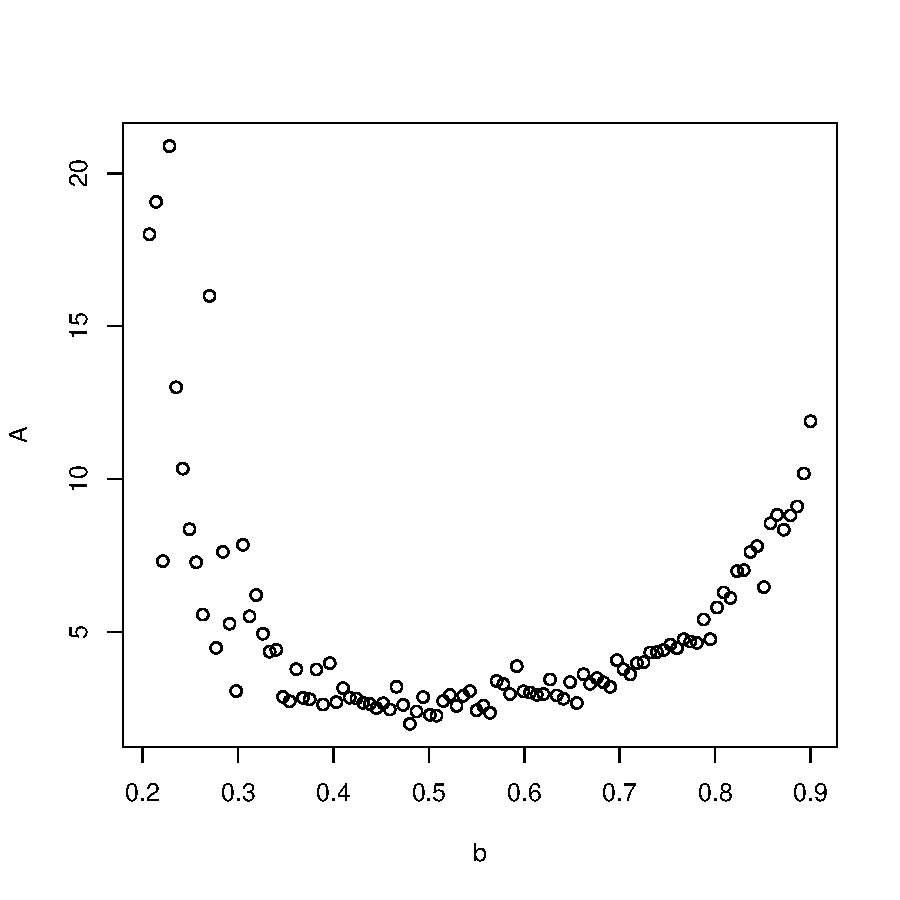
\includegraphics[width=5.0in]{Aloha1.pdf}
% }
% \caption{Scatter Plot}
% \label{scatter}
% \end{figure}
% 
% Note that though our values b here are nonrandom, the A values are
% indeed random.  To dramatize that point, I ran the program again.
% (Remember, unless you specify otherwise, R will use a different seed for
% its random number stream each time you run a program.)  I've
% superimposed this second data set on the first, using filled circles
% this time to represent the points:
% 
% \begin{Verbatim}[fontsize=\relsize{-2}]
% md2 <- alohamain(4,0.1,1000,100)
% points(md2,cex=0.5,pch=19)
% \end{Verbatim}
% 
% The plot is shown in Figure \ref{scatter2}.
% 
% \begin{figure}[tb]
% \centerline{
% \includegraphics[width=5.0in]{Aloha1a.pdf}
% }
% \caption{Scatter Plot, Two Data Sets}
% \label{scatter2}
% \end{figure}
% 
% We do expect some kind of U-shaped relation, as seen here.  For b too
% small, the nodes are clashing with each other a lot, causing long delays
% to message transmission.  For b too large, we are needlessly backing off
% in many cases in which we actually would get through.
% 
% So, a model that expresses mean A to be a linear function of b, as in
% our height-weight example, is clearly inappropriate.  However, you may
% be surprised to know that we can \underline{still} use a linear
% regression model!  And this is common.  Here are the details:
% 
% This looks like a quadratic relationship, meaning the following.  Take
% our response variable Y to be A, take our first predictor $X^{(1)}$ to
% be b, and take our second predictor $X^{(2)}$ to be $b^2$.  Then when we
% say A and b have a quadratic relationship, we mean
% 
% \begin{equation}
% \label{quad}
% m_{A;b}(b) = \beta_0 + \beta_1 b + \beta_2 b^2
% \end{equation}
% 
% for some constants $\beta_0, \beta_1, \beta_2$.  So, we are using a
% three-parameter family for our model of $m_{A;b}$.  No model is exact,
% but our data seem to indicate that this one is reasonably good, and if
% further investigation confirms that, it provides for a nice compact
% summary of the situation.  
% 
% As mentioned, this is a {\it linear} model, in the sense that the $\beta_i$
% enter into (\ref{quad}) is a linear manner.  The fact that that equation
% is quadratic in b is irrelevant.  By the way, one way to look at the
% degree-2 term is to consider it to model the ``interaction'' of b with
% itself.
% 
% Again, we'll see how to estimate the $\beta_i$ in Section \ref{parest}.
% 
% We could also try adding two more predictor variables, consisting of
% $X^{(3)} = q$ and  $X^{(4)} = s$, the node activation probability and
% number of nodes, respectively.  We would collect more data, in which we
% varied the values of q and s, and then could entertain the model
% 
% \begin{equation}
% \label{quadmore}
% m_{A;b,q}(u,v,w) = \beta_0 + \beta_1 u + \beta_2 u^2 + \beta_3 v + \beta_4 w
% \end{equation}
% 
% R or any other statistical package does the work for us.  In R, we can
% use the {\bf lm()} (``linear model'') function:
% 
% \begin{Verbatim}[fontsize=\relsize{-2}]
% > md <- cbind(md,md[,1]^2)
% > lmout <- lm(md[,2] ~ md[,1] + md[,3])
% \end{Verbatim}
% 
% First I added a new column to the data matrix, consisting of
% $b^2$.  I then called {\bf lm()}, with the argument
% 
% \begin{Verbatim}[fontsize=\relsize{-2}]
% md[,2] ~ md[,1] + md[,3]
% \end{Verbatim}
% 
% R documentation calls this model specification argument the {\bf
% formula}.  It states that I wish to use the first and third columns of
% {\bf md}, i.e. $b$ and $b^2$, as predictors, and use A, i.e. second
% column, as the response variable.\footnote{Unfortunately, R did not
% allow me to put the squared column directly into the formula, forcing me
% to use {\bf cbind()} to make a new matrix.}
% 
% The return value from this call, which I've stored in {\bf lmout}, is an
% object of class {\bf lm}.  One of the member variables of that class,
% {\bf coefficients}, is the vector $\widehat{\beta}$:
% 
% \begin{Verbatim}[fontsize=\relsize{-2}]
% > lmout$coefficients
% (Intercept)     md[, 1]     md[, 3]
%    27.56852   -90.72585    79.98616
% \end{Verbatim}
% 
% So, $\widehat{\beta}_0 = 27.57$ and so on.
% 
% The result is
% 
% \begin{equation}
% \label{quadest}
% \widehat{m}_{A,b}(t) = 27.57 - 90.73 t + 79.99 t^2
% \end{equation}
% 
% (Do you understand why there is a hat about the m?)
% 
% Another member variable in the {\bf lm} class is {\bf fitted.values}.
% This is the ``fitted curve,'' meaning the values of (\ref{quadest}) at
% $b_1,...,b_{100}$.  In other words, this is (\ref{quadest}).  I plotted
% this curve on the same graph, 
% 
% \begin{Verbatim}[fontsize=\relsize{-2}]
% > lines(cbind(md[,1],lmout$fitted.values))
% \end{Verbatim}
% 
% See Figure \ref{qc}.  As you can see, the fit looks fairly good.  What
% should we look for?
% 
% {\bf Remember, we don't expect the curve to go through the points---we
% are estimating the \underline{mean} of A for each b, not the A values
% themselves.}  There is always variation around the mean.  If for
% instance we are looking at the relationship between people heights and
% weights, the mean weight for people of height 70 inches might be, say,
% 160 pounds, but we know that some 70-inch-tall people weigh more than
% this and some weigh less.
% 
% However, there seems to be a tendency for our estimates of
% $\widehat{m}_{A,b}(t)$ to be too low for values in the middle range of
% t, and possible too high for t around 0.3 or 0.4.  {\bf However, with a
% sample size of only 100, it's difficult to tell.} It's always important
% to keep in mind that the data are random; a different sample may show
% somewhat different patterns.  Nevertheless, we should consider a more
% complex model.
% 
% \begin{figure}[tb] 
% \centerline{
% 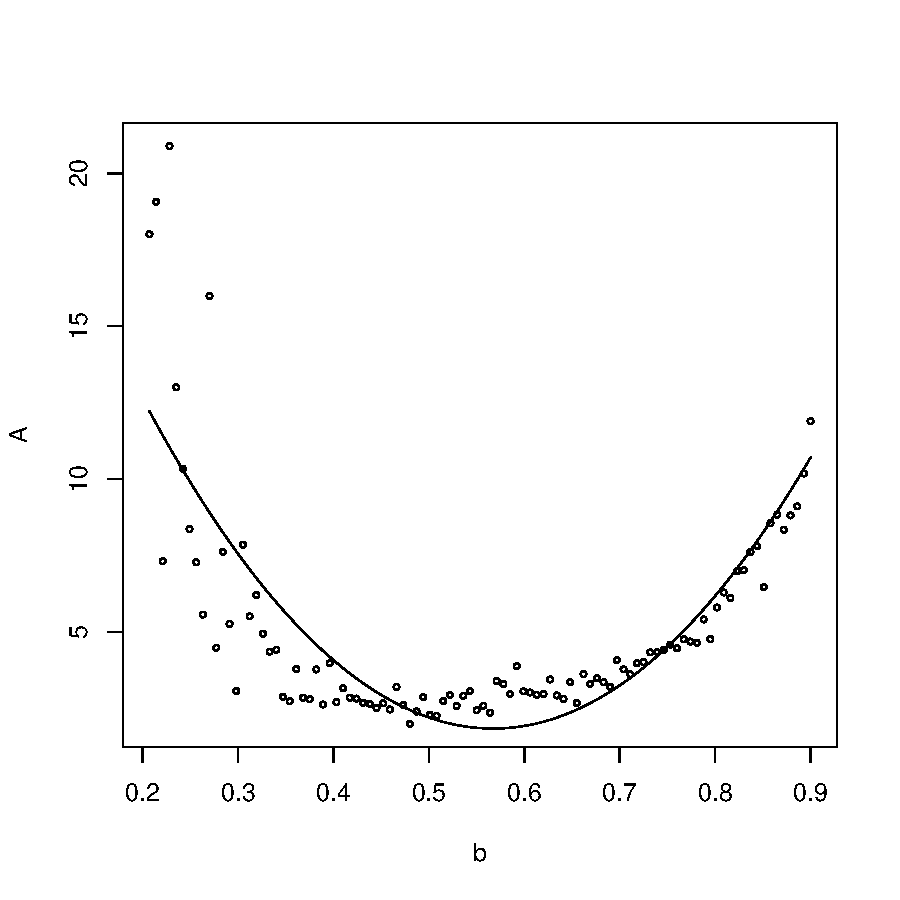
\includegraphics[width=5.0in]{AlohaFitted.pdf}
% }
% \caption{Quadratic Fit Superimposed}
% \label{qc}
% \end{figure}
% 
% So I tried a quartic, i.e. fourth-degree, polynomial model.  I added
% third- and fourth-power columns to {\bf md}, calling the result {\bf
% md4}, and invoked the call
% 
% \begin{Verbatim}[fontsize=\relsize{-2}]
% lm(md4[,2] ~ md4[,1] + md4[,3] + md4[,4] + md4[,5])
% \end{Verbatim}
% 
% The result was 
% 
% \begin{Verbatim}[fontsize=\relsize{-2}]
% > lmout$coefficients
% (Intercept)    md4[, 1]    md4[, 3]    md4[, 4]    md4[, 5]
%    95.98882  -664.02780  1731.90848 -1973.00660   835.89714
% \end{Verbatim}
% 
% In other words, we have an estimated regression function of
% 
% \begin{equation}
% \label{fourest}
% \widehat{m}_{A,b}(t) = 
% 95.98882  - 664.02780 ~ t  + 1731.90848 ~ t^2 - 1973.00660 ~ t^3  +
% 835.89714 ~ t^4
% \end{equation}
% 
% The fit is shown in Figure \ref{fourc}.  It looks much better.  On the
% other hand, we have to worry about overfitting.  We return to this issue
% in Section \ref{overfit}). 
% 
% % \checkpoint
% 
% \begin{figure}[tb] 
% \centerline{
% 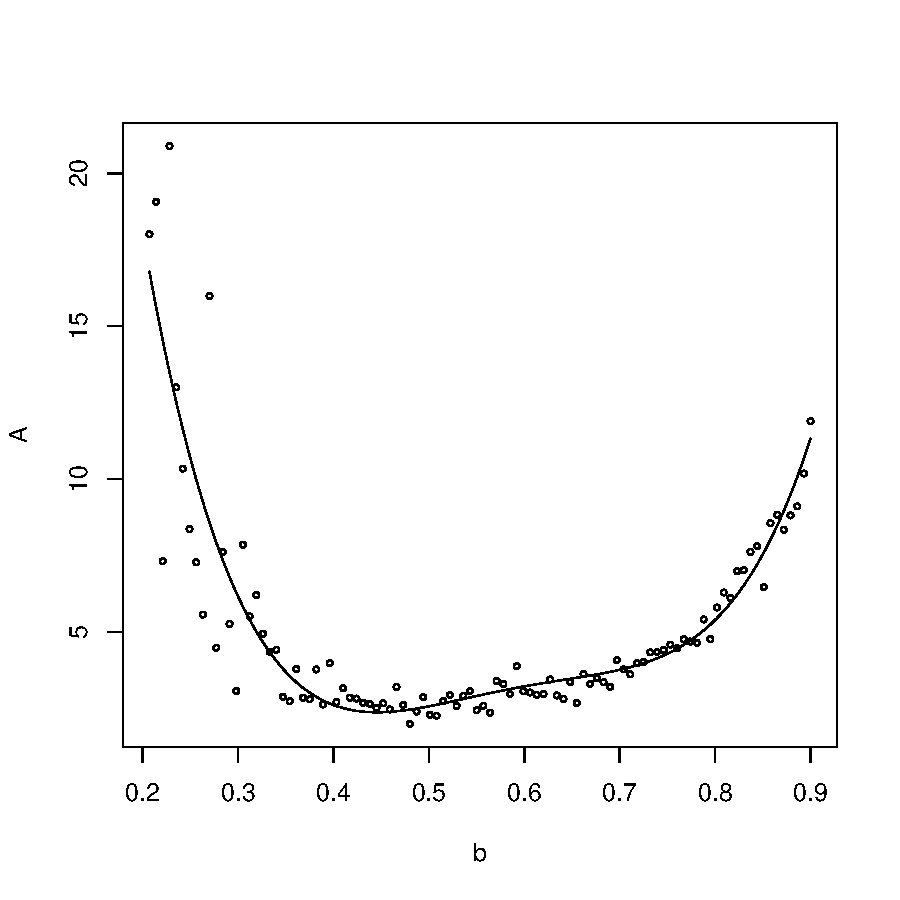
\includegraphics[width=5.0in]{AlohaFitted4.pdf}
% }
% \caption{Fourth Degree Fit Superimposed}
% \label{fourc}
% \end{figure}

\subsection{Approximate Confidence Intervals}
\label{regappcis}

As noted, R gives you standard errors for the estimated coefficients.
Where do they come from?

As usual, we should not be satisfied with just point estimates, in this
case the $\widehat{\beta}_i$.  We need an indication of how accurate
they are, so we need confidence intervals.  In other words, we need to
use the $\widehat{\beta}_i$ to form confidence intervals for the
$\beta_i$.

For instance, recall the study on object-oriented programming in Section
\ref{goals}.  The goal there was primarily Description, specifically
assessing the impact of OOP.  That impact is measured by $\beta_2$.
Thus, we want to find a confidence interval for $\beta_2$.

Equation (\ref{betahat}) shows that the $\widehat{\beta}_i$ are sums of
the components of V, i.e. the $W_j$.  So, the Central Limit Theorem
implies that the $\widehat{\beta}_i$ are approximately normally
distributed.  That in turn means that, in order to form confidence
intervals, we need standard errors for the $\beta_i$.  How will we get
them?

Note carefully that so far we have made NO assumptions other than
(\ref{linmod}).  Now, though, we need to add an
assumption:\footnote{Actually, we could derive some usable, though
messy,standard errors without this assumption.}

\begin{equation}
\label{hmsced}
Var(Y|X=t) = \sigma^2 
\end{equation}

for all t.  Note that this and the independence of the sample
observations (e.g. the various people sampled in the Davis height/weight
example are independent of each other) implies that

\begin{equation}
\label{samevar}
Cov(V|Q) = \sigma^2 I
\end{equation}

where I is the usual identiy matrix (1s on the diagonal, 0s off
diagonal).

Be sure you understand what this means.  In the Davis weights example,
for instance, it means that the variance of weight among 72-inch tall
people is the same as that for 65-inch-tall people.  That is not quite
true---the taller group has larger variance---but research into this has
found that as long as the discrepancy is not too bad, violations of this
assumption won't affect things much.

% \checkpoint

We can derive the covariance matrix of $\hat{\beta}$ as follows.  Again
to avoid clutter, let $B = (Q'Q)^{-1}$.  A theorem from linear algebra
says that Q'Q is symmetric and thus B is too.  Another theorem says that
for any conformable matrices U and V, then (UV)' = V'U'.  Armed with
that knowledge, here we go:

\begin{eqnarray}
Cov(\hat{\beta}) &=& 
Cov (
BQ'V
) ~ \textrm{((\ref{betahat}))} \\ 
&=& BQ' Cov(V) (BQ')' ~ \textrm{(\ref{covawaprime})} \\
&=& BQ' \sigma^2 I (BQ')' ~ \textrm{(\ref{samevar})} \\
&=& \sigma^2 BQ' QB ~ \textrm{(lin. alg.)} \\
&=& \sigma^2 (Q'Q)^{-1} ~ \textrm{(def. of B)} \label{betahatcov}
\end{eqnarray}


Whew!  That's a lot of work for you, if your linear algebra is rusty.
But it's worth it, because (\ref{betahatcov}) now gives us what we need
for confidence intervals.  Here's how:

First, we need to estimate $\sigma^2$.  Recall first that for any 
random variable U, $Var(U) = E[(U-EU)^2]$, we have

\begin{eqnarray}
\sigma^2 &=& Var(Y|X=t) \\
&=& Var(Y|X^{(1)}=t_1,...,X^{(r)}=t_r) \\
&=& E \left [ \{ Y - m_{Y;X}(t) \}^2 \right ] \\
&=& E \left [ (Y - \beta_0 - \beta_1 t_1 - ...  - \beta_r t_r)^2 \right ]
\end{eqnarray}

Thus, a natural estimate for $\sigma^2$ would be the sample analog,
where we replace E() by averaging over our sample, and replace
population quantities by sample estimates:

\begin{equation}
s^2 = \frac{1}{n} \sum_{i=1}^{n} 
(Y_i - \hat{\beta_0} - \hat{\beta_1} X_i^{(1)} - ...
- \hat{\beta_r} X_i^{(r)})^2 
\end{equation}

As in Chapter \ref{chap:est}, this estimate of $\sigma^2$ is biased, and
classicly one divides by n-(r+1) instead of n.  But again, it's not an
issue unless r+1 is a substantial fraction of n, in which case you are
overfitting and shouldn't be using a model with so large a value of r.

So, the estimated covariance matrix for $\hat{\beta}$ is

\begin{equation}
\label{vcov}
\widehat{Cov}(\hat{\beta}) = s^2 (Q'Q)^{-1} 
\end{equation}

The diagonal elements here are the squared standard errors (recall that
the standard error of an estimator is its estimated standard deviation)
of the $\beta_i$.  (And the off-diagonal elements are the estimated
covariances between the $\beta_i$.)  Since the first standard errors you
ever saw, in Section \ref{stderrest}, included factors like
$1/\sqrt{n}$, you might wonder why you don't see such a factor in
(\ref{vcov}).

The answer is that such a factor is essentially there, in the following
sense.  Q'Q consists of various sums of products of the X values, and
the larger n is, then the larger the elements of Q'Q are. So,
$(Q'Q)^{-1}$ already has something like a ``1/n'' factor in it.

R's {\bf vcov()} function, applied to the output of {\bf lm()} will give
you (\ref{vcov}) (subject to a bias correction factor that we'll discuss
in Section \ref{exactlinreg}, but that we'll dismiss as unimportant.

\section{Example:  Baseball Data (cont'd.)}

Let us use {\bf vcov()} to obtain the estimated covariance
matrix of the vector $\widehat{\beta}$ for our baseball data.

\begin{lstlisting}
> lmout <- lm(players$Weight ~ players$Height + players$Age)
> vcov(lmout)
               (Intercept) players$Height  players$Age
(Intercept)    320.0706223   -4.102047105 -0.607718793
players$Height  -4.1020471    0.054817211  0.002160128
players$Age     -0.6077188    0.002160128  0.015607390
\end{lstlisting}

The first command saved the output of {\bf lm()} in a variable that
we chose to name {\bf lmout}; we then called {\bf vcov()} on that
object.

For instance, the estimated variance of $\widehat{\beta}_1$ is
0.054817211.  Actually, we already knew this, because the standard error
of $\widehat{\beta}_1$ was reported earlier to be 0.2341, and
$0.2341^2 = 0.054817211$.  

But now we can find more.  Say we wish to compute a confidence interval
for the population mean weight of players who are 72 inches tall and age
30.  That quantity is equal to 

\begin{equation}
\beta_0 + 72 \beta_1 + 30 \beta_2 = (1,72,30) \beta
\end{equation}

which we will estimate by

\begin{equation}
(1,72,30) \widehat{\beta}
\end{equation}

Thus, using (\ref{quadform2}), we have

\begin{equation}
\label{cifor7230}
\widehat{Var}(\widehat{\beta}_0 + 72 \widehat{\beta}_1 + 30 \widehat{\beta}_2) =
(1,72,30) A 
\left (
\begin{array}{r}
1 \\
72 \\
30
\end{array}
\right )
\end{equation}

where A is the matrix in the R output above.

The square root of this quantity is the standard error of
$\widehat{\beta}_0 + 72 \widehat{\beta}_1 + 30 \widehat{\beta}_2$.  We
add and subtract 1.96 times that square root to $\widehat{\beta}_0 + 72
\widehat{\beta}_1 + 30 \widehat{\beta}_2$, and then have an approximate
95\% confidence interval for the population mean weight of players who
are 72 inches tall and age 30.  

\section{Dummy Variables}
\label{nominal}

Recall our example in Section \ref{examples} concerning a study of
software engineer productivity.  To review, the authors of the study
predicted $Y$ = number of person-months needed to complete the project,
from  $X^{(1)}$ = size of the project as measured in lines of code,
$X^{(2)}$ = 1 or 0 depending on whether an object-oriented or procedural
approach was used, and other variables.

As mentioned at the time, $X^{(2)}$ is an indicator variable, often
called a ``dummy'' variable in the regression context.

Let's generalize that a bit.  Suppose we are comparing two different
object-oriented languages, C++ and Java, as well as the procedural
language C.  Then we could change the definition of $X^{(2)}$ to have
the value 1 for C++ and 0 for non-C++, and we could add another
variable, $X^{(3)}$, which has the value 1 for Java and 0 for non-Java.
Use of the C language would be implied by the situation $X^{(2)} =
X^{(3)} = 0$.

Note that we do NOT want to represent Language by a single value having
the values 0, 1 and 2, which would imply that C has, for instance,
double the impact of Java.

\section{Example:  Baseball Data (cont'd.)}
\label{baseball3}

Let's now bring the Position variable into play.  First, what is
recorded for that variable?

\begin{lstlisting}
> levels(players$Position)
[1] "Catcher"           "Designated_Hitter" "First_Baseman"    
[4] "Outfielder"        "Relief_Pitcher"    "Second_Baseman"   
[7] "Shortstop"         "Starting_Pitcher"  "Third_Baseman"    
\end{lstlisting}

So, all the outfield positions have been simply labeled ``Outfielder,''
though pitchers have been separated into starters and relievers.

Technically, this variable, {\bf players\$Position}, is an R {\bf
factor}.  This is a fancy name for an integer vector with labels, such
that the labels are normally displayed rather than the codes.  So
actually catchers are coded 1, designated hitters 2, first basemen 3 and
so on, but in displaying the data frame, the labels are shown rather
than the codes.

The designated hitters are rather problematic, as they only exist in the
American League, not the National League.  Let's restrict our analysis
to the other players:

\begin{lstlisting}
> nondh <- players[players$Position != "Designated_Hitter",]
> nrow(players)
[1] 1034
> nrow(nondh)
[1] 1016
\end{lstlisting}

This requires some deconstruction.  The expression
\lstinline{players$Position != "Designated_Hitter"} gives us a vector of
True and False values.  Then
\lstinline{players[players$Position != "Designated_Hitter",]} consists
of all rows of {\bf players} corresponding to a True value.  Result:
We've deleted the designated hitters, assigning the result to {\bf
nondh}.  A comparison of numbers of rows show that there were only 18
designated hitters in the data set anyway.

Let's consolidate into four kinds of positions:  infielders,
outfielders, catchers and pitchers.  First, switch to numeric codes, in
a vector we'll name {\bf poscodes}:

\begin{lstlisting}
> poscodes <- as.integer(nondh$Position)
> head(poscodes)
[1] 1 1 1 3 3 6
> head(nondh$Position)
[1] Catcher        Catcher        Catcher        First_Baseman  First_Baseman 
[6] Second_Baseman
9 Levels: Catcher Designated_Hitter First_Baseman ... Third_Baseman
\end{lstlisting}

Now consolidate into three dummy variables:

\begin{lstlisting}
> infld <- as.integer(poscodes==3 | poscodes==6 | poscodes==7 | poscodes==9)
> outfld <- as.integer(poscodes==4)
> pitcher <- as.integer(poscodes==5 | poscodes==8)
\end{lstlisting}

Again, remember that catchers are designated via the other three dummies
being 0.

So, let's run the regression:

\begin{verbatim}
> summary(lm(nondh$Weight ~ nondh$Height + nondh$Age + infld + outfld + pitcher))

Call:
lm(formula = nondh$Weight ~ nondh$Height + nondh$Age + infld + 
    outfld + pitcher)

Residuals:
    Min      1Q  Median      3Q     Max 
-49.669 -12.083  -0.386  10.410  75.081 

Coefficients:
              Estimate Std. Error t value Pr(>|t|)    
(Intercept)  -193.2557    19.0127 -10.165  < 2e-16 ***
nondh$Height    5.1075     0.2520  20.270  < 2e-16 ***
nondh$Age       0.8844     0.1251   7.068 2.93e-12 ***
infld          -7.7727     2.2917  -3.392 0.000722 ***
outfld         -6.1398     2.3169  -2.650 0.008175 ** 
pitcher        -8.3017     2.1481  -3.865 0.000118 ***
---
Signif. codes:  0 ‘***’ 0.001 ‘**’ 0.01 ‘*’ 0.05 ‘.’ 0.1 ‘ ’ 1 

Residual standard error: 17.1 on 1009 degrees of freedom
  (1 observation deleted due to missingness)
Multiple R-squared: 0.3286,	Adjusted R-squared: 0.3253 
F-statistic: 98.76 on 5 and 1009 DF,  p-value: < 2.2e-16 
\end{verbatim}

The estimated coefficients for the position variables are all negative.
For example, for a given height and age, pitchers are on average about
8.3 pounds lighter than catchers, while outfielders are about 6.1 pounds
lighter than catchers.

What if we want to compare infielders and outfielders, say form a
confidence interval for $\beta_3 - \beta_4$?  Then we'd do a computation
like (\ref{cifor7230}), with a vector (0,0,0,1,-1,0) instead of
(1,72,30).

\section{What Does It All Mean?---Effects of Adding Predictors}

Keep in mind the twin goals of regression analysis, Prediction and
Description.  In applications in which Description is the goal, we
are keenly interested in the signs and magnitudes of the
$\beta_i$,\footnote{As estimated from the $\widehat{\beta}_i$.}
especially their signs.  We do need to be careful, just as we saw in
Section \ref{whatswrong}; the sign of a coefficient usually won't be of
much interest if the magnitude is near 0.  Subject to that caution,
discussion of regression results often centers on the sign of a
coefficient:  Is there a positive relationship between the response
variable and a predictor, holding the other predictors constant?

That latter phrase, {\it holding the other predictors constant}, is key.
Recall for example our example at the start of this chapter on a study
of the effects of using the object-oriented programming paradigm.  Does
OOP help or hurt productivity?  Since longer programs often take longer
to write, the researchers wanted to correct for program length, so they
used that as a predictor, in addition to a dummy variable for OOP.  In
other words, they wanted to know the impact of OOP on productivity,
holding program length constant.

So, in studying a predictor variable, it may matter greatly which other
predictors one is using.  Let's examine the baseball data in this
regard.

In Section \ref{baseball2}, we added the age variable as our second
predictor, height being the first.  This resulted in the coefficient of
height increasing from 4.84 to 4.97.  This is not a large change, but
what does it tell us?  It suggests that older players tend to be
shorter.  No, this doesn't mean the players shrink with age---shrinkage
does occur among the elderly, but likely not here---but rather that
other phenomena are at work.  It could be, for instance, that shorter
players tend to have longer careers.  This in turn might be due to a
situation in which certain positions whose players tend to be tall have
shorter careers.  All of this could be explored, say starting with
calculating the correlation between height and age.\footnote{The R
function {\bf cor()} computes the correlation between its first two
arguments if they are vectors.}

To develop some intuition on this, consider the following artificial
population of eight people:

\bigskip

\begin{tabular}{|r|r|r|}
\hline
gender & height & weight \\ \hline 
male & 66 & 150 \\ \hline 
male & 70 & 165 \\ \hline 
male & 70 & 175 \\ \hline 
male & 70 & 185 \\ \hline 
female & 66 & 120 \\ \hline 
female & 66 & 130 \\ \hline 
female & 66 & 140 \\ \hline 
female & 70 & 155 \\ \hline 
\end{tabular}

\bigskip

Here is the weight-height relationship for men, i.e. the mean weight for
each height group:

\bigskip

men:

\begin{tabular}{|r|r|}
\hline
height & mean weight \\ \hline 
66 & 150 \\ \hline 
70 & 175 \\ \hline 
\end{tabular}

\begin{equation}
\beta_{height} = (175-150) / 4 = 6.25
\end{equation}

women:

\begin{tabular}{|r|r|}
\hline
height & mean weight \\ \hline 
66 & 130 \\ \hline 
70 & 155 \\ \hline 
\end{tabular}

\begin{equation}
\beta_{height} = (155-130) / 4 = 6.25
\end{equation}

\bigskip

The coefficient of height is the same for both gender subpopulations.

But look what happens when we remove gender from the analysis:

\bigskip

all:

\begin{tabular}{|r|r|}
\hline
height & mean weight \\ \hline 
66 & 135 \\ \hline 
70 & 170 \\ \hline 
\end{tabular}

\begin{equation}
\beta_{height} = (170-135) / 4 = 8.75
\end{equation}

In other words, the beta coefficient for height is 8.75 if gender is not
in the equation, but is only 6.25 if we add in gender.  For a given
height, men in this population tend to be heavier, and since the men
tend to be taller, that inflated the height coefficient in the
genderless analysis.

Returning to the baseball example, recall that in in Section
\ref{baseball3}, we added the position variables to height and age as
predictors.  The coefficient for height, which had increased when we
added in the age variable, now increased further, while the coefficient
for age decreased, compared to the results in Section \ref{baseball2}.
Those heavy catchers weren't separated out from the other players in our
previous analysis, and now that we are separating them from the rest,
the relationship of weight versus height and age is now clarified.

Such thinking was central to another baseball example, in {\it Mere
Mortals:  Retract This Article}, Gregory Matthews blog, 

\url{http://statsinthewild.wordpress.com/2012/08/23/mere-mortals-retract-this-article/}.

There the author took exception to someone else's analysis that
purported to show that professional baseball players have a higher
mortality rate than do pro football players.  This was counterintuitive,
since football is more of a contact sport.  It turned out that the
original analysis had been misleading, as it did not use age as a
predictor.

Clearly, the above considerations are absolutely crucial to effective
use of regression analysis for the Description goal.  This insight is
key---don't do regression without it!  And for the same reasons,
whenever you read someone else's study, do so with a skeptical eye.

% \subsection{Once Again, Our ALOHA Example} 
% 
% In R we can obtain (\ref{vcov}) via the generic function {\bf vcov()}:
% 
% \begin{Verbatim}[fontsize=\relsize{-2}]
% > vcov(lmout)
%             (Intercept)    md4[, 1]   md4[, 3]   md4[, 4]   md4[, 5]
% (Intercept)    92.73734   -794.4755   2358.860  -2915.238   1279.981
% md4[, 1]     -794.47553   6896.8443 -20705.705  25822.832 -11422.355
% md4[, 3]     2358.86046 -20705.7047  62804.912 -79026.086  35220.412
% md4[, 4]    -2915.23828  25822.8320 -79026.086 100239.652 -44990.271
% md4[, 5]     1279.98125 -11422.3550  35220.412 -44990.271  20320.809
% \end{Verbatim}
% 
% What is this telling us?  For instance, it says that the (4,4) position
% (starting at (0,0) in the matrix (\ref{vcov}) is equal to 20320.809, so
% the standard error of $\widehat{\beta}_4$ is the square root of this,
% 142.6.  Thus an approximate 95\% confidence interval for the true
% population $\beta_4$ is
% 
% \begin{equation}
% \label{bigci}
% 835.89714 \pm 1.96 \cdot 142.6 = (556.4,1115.4)
% \end{equation}
% 
% That interval is quite wide.  The margin of error, $1.96 \cdot 142.6 =
% 279.5$ is more than half of the left endpoint of the interval, 556.4.
% Remember what this tells us---that our sample of size 100 is not very
% large.  On the other hand, the interval is quite far from 0, which
% indicates that our fourth-degree model is substantially better than our
% quadratic one.  
% 
% Applying the R function {\bf summary()} to a linear model object such as
% {\bf lmout} here gives standard errors for the $\widehat{\beta}_i$ (and
% lots of other information), so we didn't really need to call {\bf
% vcov()}.  But that call can give us more:
% 
% Note that we can apply (\ref{covawaprime}) to the estimated covariance
% matrix of $\widehat{\beta}$!  Recall our old example of measuring
% the relation between people's weights and heights, 
% 
% \begin{equation}
% m_{W;H}(t) = \beta_0 + \beta_1 t
% \end{equation}
% 
% Suppose we estimate $\beta$ from our data, and wish to find a confidence
% interval for the mean height of all people of height 70 inches, which is
% 
% \begin{equation}
% \beta_0 + 70 \beta_1
% \end{equation}
% 
% Our estimate is
% 
% \begin{equation}
% \label{estmean70}
% \widehat{\beta}_0 + 70 \widehat{\beta}_1
% \end{equation}
% 
% That latter quantity is 
% 
% \begin{equation}
% (1,70) \widehat{\beta}
% \end{equation}
% 
% perfect for (\ref{genmvci}).  Thus
% 
% \begin{equation}
% \widehat{Var}(\widehat{\beta}_0 + 70 \widehat{\beta}_1) =
% (1,70) C
% \left (
% \begin{array}{r}
% 1 \\
% 70 \\
% \end{array}
% \right )
% \end{equation}
% 
% where C is the output from {\bf vcov()}.  The square root of this is
% then the standard error for (\ref{estmean70}).  (Recall Section
% \ref{stderrest}.)

% \checkpoint

% \subsection{Estimation Vs. Prediction} 
% 
% In statistical parlance, there is a keen distinction made between the
% words {\it estimation} and {\it prediction}.  To explain this, let's
% again consider the example of predicting Y = weight from X =
% (height,age).  Say we have someone of height 67 inches and age 27, and
% want to guess---i.e. {\it predict}---her weight.
% 
% From Section \ref{optimal1}, we know that the best prediction is
% m[(67,27)].  However, we do not know the value of that quantity, so
% we must {\it estimate} it from our data.  So, our {\it predicted value}
% for this person's weight will be $\hat{m}[(67,27)]$, i.e. our {\it
% estimate} for the value of the regression function at the point (67,27).

